\documentclass[a4paper,notitlepage]{article}

\usepackage[top=2cm, bottom=2cm, left=3cm, right=3cm]{geometry}

\usepackage{float}

\usepackage{multirow}

\usepackage[hyphens]{url}
\usepackage{hyperref}

\usepackage{appendix}
\usepackage[numbers]{natbib}

\usepackage{graphicx}
\usepackage{epstopdf}

\usepackage{tabularx}

\usepackage[parfill]{parskip}
\setlength{\parindent}{0pt}
\setlength{\parskip}{\baselineskip}

% A better tilde (~)
\newcommand{\mytilde}{\raise.17ex\hbox{$\scriptstyle\mathtt{\sim}$} }

% For use in the title page
\newcommand{\HRule}{\rule{\linewidth}{0.5mm}}


% For \begin{acknowledgements}
% From: http://www.latex-community.org/forum/viewtopic.php?f=47&t=5464
\makeatletter
\newcommand\ackname{Acknowledgements}
\if@titlepage
  \newenvironment{acknowledgements}{%
      \titlepage
      \null\vfil
      \@beginparpenalty\@lowpenalty
      \begin{center}%
        \bfseries \ackname
        \@endparpenalty\@M
      \end{center}}%
     {\par\vfil\null\endtitlepage}
\else
  \newenvironment{acknowledgements}{%
      \if@twocolumn
        \section*{\abstractname}%
      \else
        \small
        \begin{center}%
          {\bfseries \ackname\vspace{-.5em}\vspace{\z@}}%
        \end{center}%
        \quotation
      \fi}
      {\if@twocolumn\else\endquotation\fi}
\fi
\makeatother


\title{Towards Debugging Wireless Sensor Network Applications}
\date{October 2012 - July 2013}
\author{
	Matthew Bradbury (0921660) \and
	Tim Law (0918647) \and
	Ivan Leong () \and
	Daniel Robertson (0910210) \and
	Amit Shah (0904778) \and
	Joe Yarnall (0905247)
}
\begin{document}

\begin{titlepage}
\begin{center}

% Upper part of the page

\includegraphics[scale=1.15]{the_warwick_uni_blue.eps}\\[0.75cm]

\textsc{\LARGE Department of Computer Science}\\[1.5cm] 

\textsc{\Large Fourth Year Project}\\[0.5cm]


% Title
\HRule \\[0.4cm]
{\Huge \bfseries Towards Debugging Wireless Sensor Network Applications}\\[0.4cm]

\HRule \\[2cm]

% Author and supervisor
\noindent{
\begin{minipage}{0.4\textwidth}
\begin{flushleft} \large
\emph{Authors:}\\
Matthew Bradbury (0921660) \\
Tim Law () \\
Ivan Leong (0830934) \\
Daniel Robertson (0910210) \\
Amit Shah (0904778) \\
Joe Yarnall (0905247)\\
\end{flushleft}
\end{minipage}}
\hfill
\noindent{
\begin{minipage}{0.4\textwidth}
\begin{flushright} \large
\emph{Supervisor:} \\
Dr.~Arshad Jhumka
\end{flushright}
\end{minipage}}

\vfill

\begin{abstract}
Abstract
\newline
\newline
\noindent \textbf{Keywords} - Wireless Sensor Networks; Debugging; Global Predicate Detection;
\end{abstract}

\vfill
\vfill
\vfill
\vfill

% Bottom of the page
{\large October 2012 - July 2013}

\end{center}
\end{titlepage}

%No numbering on first and second pages
\pagestyle{empty}
\thispagestyle{empty}

\newpage

\begin{acknowledgements}
Acknowledgements
\end{acknowledgements}
\newpage


\pagestyle{plain}
\setcounter{page}{1}

\tableofcontents
\clearpage


% !TeX root = Report.tex
\section{Introduction}

\subsection{What is a Wireless Sensor Network?}

A wireless sensor network, or WSN for short, is a collection of networked sensors called Motes; these sensors are capable of short range wireless communication and they have the ability to sense their surrounding environment\cite{Mica2002,TankBible}. The network forms a distributed system that can perform a variety of distributed algorithms, usually data gathering and similar tasks. To communicate, each node is equipped with a radio that allows them to send and receive messages to neighbouring nodes within a limited range. To sense the environment motes typically have a range of embedded sensors such as heat, light, humidity and many others. They typically contain a simple central processing unit (CPU), which is programmed to control the hardware on the motes. The CPU also processes events which are triggered by the hardware (such as messages being sent and received) and it also handles any other computation necessary for the operation of the system. As the platform is designed to be mobile the motes do not operate on a mains power supply, instead they run off stored energy in a battery. WSNs is a field of Computer Science that is currently the focus of much research and wireless sensor networks have a wide range of practical applications that stretch from battlefield intelligence for the military\cite{?} to industrial process monitoring for manufacturing companies\cite{?}.

A defining characteristic of designing applications for wireless sensor networks is the restricted and finite energy supply available to each node. Therefore, wireless sensor nodes tend not to use expensive broadcasting protocols such as IEEE 802.11 \cite{Mica2002}, but instead use much simpler alternatives to save energy. For example wireless protocols such as IEEE 802.15.4 ZigBee \cite{1253873, 4014617} are designed to be used by wireless sensor networks and have a lower energy usage associated with them. Some applications rely on even lower level behaviour specified by a certain MAC layer \cite{5751321,4469515,?,BMAC,SMAC,XMAC}, these applications involve a trade-off between development time and energy usage. Where simplicity is often sacrificed for decreased energy usage. Using these simple protocols unfortunately has the downside of meaning that broadcasts are subject to several types of collisions and message losses. So it is very important that the software running on the nodes is designed to handle these cases. Being battery powered means that development of applications for Wireless Sensor Networks is fundamentally limited to maximising the system's lifetime so that the highest utility can be achieved from the network.

As wireless sensor nodes operate in harsh outdoors condition\cite{SzewczykPMC04, Werner-Allen:2006:FYV:1298455.1298491}, there is a high probability of them failing. These faults can range from hardware damage caused by environmental conditions or tampering, software bugs, or simply a denial of service caused by nodes running out of power. So algorithms and software need to be designed to handle these potential failures, otherwise they risk catastrophic failure when they encounter these issues.

Wireless sensor nodes are designed with the intention for them to operate in remote and traditionally unreachable locations with no human input for the lifetime of their operation\cite{1437066}. Given this a defining characteristic of a WSN system is that any applications developed for it must be self-configuring in nature; this is, the system must be able to organize itself and the network with no external input\cite{?}. Evidently, solutions to this issue are often considered hand in hand with the problem of network robustness and fault tolerance.   

While a limited energy source, self-configuration and network robustness are the predominant characteristic of a wireless sensor node, there are numerous other traits or issues that can be considered. For instance it is possible for these nodes to be mobile (for example an ad-hoc network of PDAs or motes built into soldiers helmets) \cite{4224091}, this can lead to very interesting behaviour in handling communication between these nodes.

%TODO: MORE OBSCURE WSN BEHAVIOUR CONSIDERATIONS

\subsection{The Problem - Debugging Distributed Systems}

Developing a distributed system is considered a particularly challenging task, more so than a traditional application, there are several reasons for this. Firstly, Within a distributed system multiple processes must execute in parallel, this means that variables may be updated independently or in repose to other processes which can lead to a myriad of synchronisation and timing issues that the developer must account for. Secondly, traditional programming languages are not well suited to develop distributed programs\cite{93692,345131}.

In any system, software or otherwise, developed by humans there is the potential for mistakes. Mistakes can be benign or they can cause unintended behaviour and system failures. Developing tools to detect these \emph{bugs} and notify the developer so they can be corrected is an incredibly important part of any toolchain. For example the GNU toolchain has utilities such as gdb\cite{?}, this allows developers to place breakpoints in code which will halt the programs execution at that state so that it can be examined. There are also numerous other tools that look for memory issues (valgrind\cite{?}), security flaws (TOOL NAME\cite{?}) and many other classes of bugs.

Developing distributed systems is a difficult task; however, debugging these systems can be even more challenging\cite{345131}. When considering a distributed system if you want to examine the state of a system at a given point you cannot simply set a breakpoint in your local binary. The solution to this debugging is non-trivial, this is due to the difficulties that arise from distributed systems being non-deterministic in nature due to message communications \cite{?}. Be it when the message started transmission, how long it took, if it succeeded or in what order transmissions occurred. So every time a distributed program is run it is possible for a different result to be obtained, due to the different order of execution. This goes against one of the usual assumptions of debugging traditional applications where it is assumed that one execution with a set of inputs will execute in exactly the same way again with the same set of inputs\cite{?} (i.e. determinism).

As the execution may be different each time in a distributed system it is not suitable to wait for a bug to occur, and then try to work out where it is. Rather, the system needs to be self-evaluating its state as it executes the distributed program; if a fault is detected, then the debugging tools will report the issue. One way to do this it to test if the system satisfies some global predicate, of which there has been much work to find and check different classes of these predicates \cite{553309,345831,277788}. However, of all the work that has been done, little of it has focused on wireless sensor networks where an important focus is perhaps the trade-off between accuracy and the report-ability of a predicate with the aim of reducing energy usage. In this paper we will discuss our development of just such a set of tools, we intend to focus on developing a system that can accurately evaluate predicates and provide useful information about real sensor networks running outside of a simulator.

\subsection{Related Work - New Lit Review???}

\subsubsection*{Fault-Error-Failure Cycle - NEEDS WORK}

It should be clear that the types of predicates are important to consider when developing a predicate checking mechanism. Also important are the types of errors that these predicate checking algorithms can detect. To understand this it is first important to understand how errors can arise, which can be done by examining the fault-error-failure cycle. This cycle says that a \emph{fault} once caused by either some external influence (e.g. radiation leading to bit-flips in memory \cite{1017791}) or internal influence (e.g. code bugs) will lead to an \emph{error}, this is the \emph{activation} step. An error is the manifestation of the fault (e.g. memory holding the incorrect value). An error then leads to a \emph{failure} in the step called \emph{propagation}, the failure of the system is an observable deviation from the system's specification (e.g. allowing doors to be opened that should remain closed). It is not always the case the faults lead to errors, or errors lead to failures, sometimes multiple faults or errors are respectively required to cause a single error or failure. \cite{1335465}

There is a choice of what should be measured and checked in predicates; should faults, errors or failures be measured? Faults cannot be measured \cite{?} in a way that is possible for a mote, so they are discounted. That leaves measuring errors and failures. Typically failures would be the event being measured \cite{?} as that is what arises after an error actually causes the issue to happen. However, errors can also be measured if there is a dedicated program checking the state and comparing it to an expected state \cite{?}. For example an ECC (error correcting code) such as a Hamming Code can be used to detect and correct an error (in this case a bit-flip) in some memory after a fault (such as a voltage surge ) \cite{hamming1950error}.

Much of what has been discussed has involved transient faults such as those caused by environmental conditions, however, there is a class of faults that are a lot more common and much easier to resolve - faults caused by software bugs. These faults can lead to programs ending up in the wrong state and performing incorrectly. There has been a certain amount of work that looks into detecting traditional distributed system bugs (such as deadlock \cite{5587352,5284172}) in wireless sensor networks. However, there has been little work in looking into providing tools to aid in system debugging.

\subsubsection*{Classes of Distributed Predicates - NEEDS WORK}

To begin with it is important to understand what predicates are relevant to distributed systems. First off we have a distinction between global and local predicates, global predicates involve taking a consistent global snapshot of the system and checking whether the snapshot satisfies the global predicate \cite{277788} and local predicates instead work with a subset of the network \cite{553309}. These predicates have also have a notion of stability, a stable predicate will remain true once it has turned true (e.g. termination), whereas unstable predicates can alternate between true and false. Finally there is a distinction between weak and strong, where a weak predicate holds if there exists an observation where the predicate is true and a strong predicate holds if it is true for all observers of the distributed computation\cite{553309,Cooper:1991:CDG:127695.122774}. Knowing what classes of predicates there are is important because when checking certain properties of a system a certain class of predicate will be required and thus a certain implementation will be needed to ensure the predicate is correctly checked. An example of this is when running an algorithm using global snapshots to detect stable predicates, that same application may not be suitable to detect unstable predicates because the predicate could switch to false and then back to true before the next snapshot.

\subsubsection*{Existing Sensor Network Predicate Checking Tools}


\subsubsection*{Practical Sensor Network Deployments}





\clearpage

\section{Required Tools}

A simulator and operating system needs to be chosen that will allow us to test our code locally, then provide functionality to deploy that code to the network easily. We will now provide a comparison between the two primary operating systems, Contiki \cite{23839452} and TinyOS \cite{levis2003tossim}, and their respective simulators with a view to deciding which system best suits this projects goals and motivations.

TinyOS and it's simulator TOSSIM were originally created at UC Berkeley as part of the DARPA NEST Program. TinyOS is a static system where designers must allocate resources during design-time. TinyOS is also a monolithic system, in this system programs are compiled with the OS code and distributed to network nodes together as one image.

Contiiki was developed by Adam Dunkels and is an open source operating system designed for the Internet of Things. Contiki is a dynamic system that allows resources to be allocated and deallocated at run-time. Contiki is a modular system where programs are compiled into an individual module that can be distributed to the network nodes which run the code dynamically.

Both systems are event driven, however Contiki also offers native multi-threading support through proto-threads where as TinyOS does not and requires a library to gain access to threading through TinyThreads \cite{?}. TinyOS programs are implemented in nesC a variation of C designed for the TinyOS platform. The simulator COOJA can run both C and Java code but the Contiki OS can only run C code. Both systems use custom wireless networking stacks that are optimised for low power consumption. In a comparison of energy and time efficiency between Contiki and TinyOS \cite{?} it is shown that the differences between the two operating systems is negligible. The study found that Contiki is quicker at sensing, TinyOS is faster at communication between nodes and they are both equally efficient at processing tasks such as executing security algorithms.

We have chosen to use Contiki and COOJA for this project because it provides the most flexible system for developing applications that can quickly and easily be distributed to the network. Contiki also offers an easy to use fully functioning development environment and simulator tool all in one package. Finally, Contiki is almost as efficient as TinyOS in nearly every respect but provides all the additional features of a modular dynamic operating system and for these reasons this is why we have chosen it as the system we will develop for.  


\section{Knowledge Gained}
\begin{enumerate}
	\item Not possible to write WSN applications in Java and have them run on the WSN nodes. Only possible to write in C and have that code run on the physical hardware. Java code will only run in the Cooja simulator for the Contiki OS.
	\item A Cooja plug-in that monitors and records network traffic would be specific only to the simulator and would not be possible to apply to physical nodes
	\item Had to convert from raw sensor data to expected results using equations found in \cite{sensiriondatasheet}
\end{enumerate}
\clearpage


\section{Project Management}

\subsection{Work Overview}

% TODO: Convert this to a table that can flow over multiple pages
\begin{table}[H]
	\centering
	\begin{tabular}{| l | p{7.5cm} | p{5cm} |}
	Week & Activities & Task Allocation\\
	\hline
	1 & \begin{enumerate}
			\item Met up with Supervisor and discussed project direction
			\item Decided to research what has been done and what we could do, before settling on main aims
			\item Investigated two OSes and their corresponding simulators TinyOS with TOSSIM and Contiki with Cooja
		\end{enumerate} &
	\begin{enumerate}
		\item[] Amit: 1, 2, 3
		\item[] Dan: 1, 2, 3
		\item[] Ivan: 1, 2, 3
		\item[] Joe: 1, 2, 3
		\item[] Matt: 1, 2, 3
		\item[] Tim: 1, 2, 3
	\end{enumerate}
	\\ \hline

	2 & \begin{enumerate}
			\item Research if Cooja can be extended through the use of plug-ins (with the aim of extending it to replay traffic logs)
			\item Research Clustering algorithms and find implementations
			\item Develop a temperature dissemination application to learn Contiki and Cooja
			\item Research TinyOS and TinyDB and see if they could be applied to predicate checking
			\item Investigate performance of different MAC protocols
			\item Investigate the feasibility of live monitoring of the network
			\item Investigate QoS and how it may be applied to real life WSN deployments
			\item Produce a literature review on chosen topic
		\end{enumerate} &
	\begin{enumerate}
		\item[] Amit: 1, 7, 8
		\item[] Dan: 5, 8
		\item[] Ivan: 6, 8
		\item[] Joe: 4, 8
		\item[] Matt: 3, 8
		\item[] Tim: 2, 8
	\end{enumerate}
	\\ \hline
	
	3 & \begin{enumerate}
			\item Research DICAS
			\item Research Send to Base
			\item Research Daicon
			\item Research DIDUCE
			\item Research H-SEND
			\item Research Sympathy
			\item Write Specification
		\end{enumerate} &
	\begin{enumerate}
		\item[] Amit: 2, 7
		\item[] Dan: 4, 7
		\item[] Ivan: 3, 7
		\item[] Joe: 1, 7
		\item[] Matt: 6, 7
		\item[] Tim: 5, 7
	\end{enumerate}
	\\ \hline

	\end{tabular}
\end{table}

\subsection{Role Allocation}

We decided to allocate roles in the second week after we had the first week to perform research into the problem and find out what has been done. The following were how we assigned roles, although we intend for these to be flexible:

\begin{table}[H]
	\centering
	\begin{tabular}{| l | l |}
	Name & Role \\
	\hline
	Amit & ~ \\
	Dan & ~ \\
	Ivan & ~ \\
	Joe & ~ \\
	Matt & ~ \\
	Tim & ~ \\
	\end{tabular}
\end{table}


\subsection{Schedule}


\begin{table}[H]
	\centering
	\begin{tabular}{| l | l | l | l | l | l | l |}
	Task Description & \multicolumn{6}{|l|}{Time Allocated (Weeks)}\\
	~ & Amit & Dan & Ivan & Joe & Matt & Tim \\
	\hline
	\hline
	\multicolumn{7}{|l|}{\textbf{Term 1} - Developing for stationary networks} \\
	\hline


	Research around the Problem & 2 & 2 & 2 & 2 & 2 & 2\\
	Writing Specification & 1 & 1 & 1 & 1 & 1 & 1\\
	Algorithm Development & 3 & 3 & 3 & 3 & 3 & 3\\
	Testing & 1 & 1 & 1 & 1 & 1 & 1\\
	Testing and adapting to Physical Nodes & 2 & 2 & 2 & 2 & 2 & 2\\
	Poster Creation and Presentation preparation & 1 & 1 & 1 & 1 & 1 & 1\\

	\hline
	\hline
	\multicolumn{7}{|l|}{\textbf{Term 2} - Developing for mobile networks} \\
	\hline
	
	Additional Research & 1 & 1 & 1 & 1 & 1 & 1\\
	Algorithm Development & 3 & 3 & 3 & 3 & 3 & 3\\
	Testing & 2 & 2 & 2 & 2 & 2 & 2\\
	Testing and adapting to Physical Nodes & 2 & 2 & 2 & 2 & 2 & 2\\
	Report Writing & 2 & 2 & 2 & 2 & 2 & 2\\
	
	\hline
	
	\end{tabular}
\end{table}



\subsection{Working Concurrently}

We signed up for a Git repository on BitBucket \cite{?} where we plan to commit all the work we produce. We initially had an issue that free private repositories hosted on BitBucket have a maximum of 5 participants, whereas we had 6 group members. Fortunately when new users sign up to the services from an invite, the person that sends the invite gets additional capacity. This meant that the person who created the repository ended up with enough capacity for all members to access the account.

\subsection{Group Members Without Internet}
Unfortunately two of our group members were without internet for the first 3 weeks of term. This was an issue because they were unable to just work in the DCS labs because the computers there didn't have the software required (such as VirtualBox or the WSN simulators). To work around this, those two members were given tasks that could be accomplished with their own machines and without internet. Once they obtained internet they were given tasks, that access allowed them to accomplish.


\clearpage

% !TeX root = Report.tex
\section{Literature Review}

\subsection{Routing in Sensor Networks}

\subsubsection{Flooding}



\subsection{Simulating Sensor Networks}

\subsubsection{TinyOS}

\subsubsection{Contiki}
% Cite basically all the papers at: http://www.contiki-os.org/support.html

\subsubsection{NS2}

\subsubsection{JProwler}

\subsubsection{Simulating Energy Consumption}
\cite{Shnayder04}


\subsection{Sensor Network Platforms}

\subsubsection{MICA}
\cite{Mica2002}

\subsubsection{Sky}


\subsection{Practical Experience in Sensor Networks}

\subsubsection{Air Pollution}
\cite{libeliumAirPollution}
\cite{wsnpollution}

\subsubsection{Forest Fires}
\cite{libeliumForestFires}

\subsubsection{Great Duck Island}
\cite{SzewczykPMC04}

\subsubsection{Volcano Monitoring}
\cite{Werner-Allen:2006:FYV:1298455.1298491}

\subsubsection{Structural Monitoring}
\cite{5508230}

\subsubsection{Development of Applications}
\cite{Fagerstrom:1988:DTD:55823.55833}


\subsubsection{Power Considerations}


\subsection{Predicates}



\begin{comment}
\subsection{Quality of Service}
The area of Quality of Service (QoS) within Wireless Sensor Networks (WSN) is largely unexplored, due to the large differences between WSNs and traditional wireless networks. Traditional networks determine QoS based on high bandwidth allowance, as a result of high multimedia demands of applications. WSNs typically do not need to transfer this amount of data, and have a much lower bandwidth because of this. WSNs also have a wide range of different applications, and as a result, it is not clear how to develop transferable approaches to QoS  \cite{Akyildiz2002393}. 

QoS can be reduced to 'a set of service requirements to be met when transporting a packet stream from the source to its destination' \cite{Crawley98aframework}. With traditional networks, redundancy is often introduced to allow for high load/traffic, however redundancy in WSNs can often mean wasted energy usage which is often the main QoS measure in many protocols \cite{AkkayaYounis2003}.

Akyildiz et. al. \cite{Akyildiz2002393} suggested that QoS could be measured in two ways Application and Network. The Application defines measures such as coverage, number of active sensors and exposure, while the Network is concerned with delivering the QoS constrained data, while maintaining network efficiency (minimising resources).

Akyildiz et. al. further went on to describe the challenges specific to WSN; 
\begin{itemize}  
			\item Resource Constraints - Battery life, memory, bandwidth etc
			\item Unbalanced traffic - Traffic flows from large set of sensors into a small set of sink nodes
			\item Data redundancy - The re-transmission of data could result in wasted energy usage
			\item Network Dynamics - Failing nodes/wireless links, energy conservation, mobility etc
			\item Scalability 
			\item Multiple sink nodes - Each node could have a different set of requirements
			\item Packet Critically - Some data may need to flow through the network quicker than other pieces
			\item Multiple traffic types - Different pieces of data flowing through the network at the same time
\end{itemize}

QoS is a difficult term to define, mainly due to its various meanings and perspectives, because of this, measurements of quality must be generated based on the application involved, and the specific requirements of that application.


\subsection{MAC Protocols}

\subsubsection*{Energy-efficient MAC Protocol Designed for WSN for IoT (The submarine paper)}

\cite{6128220} discusses the energy efficiency of existing protocols, including the original adaptation of MAC for WSNs - Sensor MAC (SMAC). Describes the operation of SMAC, which uses a fixed listen/sleep cycle to reduce idle listening time and thus save energy. Goes on to mention two improvements on SMAC: first Timeout MAC (TMAC), in which the listen/sleep cycle is adapted according to network traffic, by means of a simple timeout mechanism; then $\mu$-MAC, which alters between contention and contention-free periods. The former is used to establish network topology and initialise sub-channels (collections of time slots), which are used in the contention-free period to transmit without collisions.

The authors then propose a power-controlled MAC protocol (PC-MAC), which determines the required transmission power level for a packet, thus aiming to save unnecessary energy usage when sending over short distances. This calculation assumes the physical layer of the nodes can transmit frames at one of a discrete set of power levels notified by the MAC layer. Once calculated, the minimum required power for each of a node's neighbours is stored in that node's Schedule and Power Level Table, an extension of the Schedule Table used for synchronising sleep cycles in SMAC. The protocol preserves the collision- and overhearing-avoidance properties of SMAC.
Authors report energy savings of between 50\% and 96\% for average node distances ranging from 10m down to 1m. These findings were generated solely using simulations, but assuming they hold for a hardware WSN the benefits for energy efficiency are significant enough to warrant serious consideration.


\subsubsection*{Energy Analysis of Four WSN MAC Protocols}

Four power-aware protocols based on the MAC framework implemented in TinyOS on TelosB motes and were tested using broadcast, convergecast and local gossip traffic patterns \cite{5751321}. Motivation: testing of the protocols side-by-side under controlled parameters, to rule out the innumerable extraneous factors that make direct comparison of separately-published protocols difficult.

Outlines history of power-saving MAC strategies, beginning with the duty cycles as described above in the operation of SMAC. Then describes the next development --- low-power listening (LPL), using transmission preambles and channel polling to reduce idle listening times. More advanced protocols use a hybrid of these two techniques.

Protocols tested:
\begin{enumerate}
	\item Scheduled Channel Polling MAC (SCP-MAC):
	\begin{itemize}
		\item Modification of LPL by waking up all neighbouring motes to listen at the same time. This leads to shorter preambles and duty cycles than typical LPL protocols (i.e. BMAC). However, all neighbours share a listening slot, so overhearing is common.
	\end{itemize}
	
	\item Asynchronous Schedules MAC (AS-MAC):
	\begin{itemize}
		\item Eliminates overhearing by assigning unique time slots for each mote to listen; the times when each mote wakes up to transmit/receive are determined by its internal Neighbour Table. At each wakeup, a mote polls for packet receptions, and motes transmit during a contention window overlapping with this wakeup slot. Loss of contention signals a retry during the recipient's next wakeup. AS-MAC uses sync packets and non-uniform offsets to offer unique receiver receptions slots, even in dense neighbourhoods.
	\end{itemize}
	
	\item Crankshaft:
	\begin{itemize}
		\item Similar to AS-MAC in that time is divided into frames, which are sub-divided into receiver slots. Frames include broadcast and unicast slots such that all neighbouring motes wake up for the all of the former, and only their own unicast slot. The ratio between the two types of slot is configurable at compile time, and the number of unicast slots is independent of the number of motes. As such, dense WSNs often feature multiple receivers contending for receptions during the same slot; clock synchronization in Crankshaft relies upon upper layers.
	\end{itemize}
	
	\item Broadcastable AS-MAC (BAS-MAC):
	\begin{itemize}
		\item During implementation of broadcasting in AS-MAC (using multiple unicast transmissions), it was noticed that a broadcasting mote must stay awake for the duration of every receive slot in the network; for nontrivial network sizes, this would be infeasible. As such, a separate protocol was created. BAS-MAC is based heavily on AS-MAC, but defines a broadcast interval; a time slot during which all neighbouring motes wake up simultaneously.
	\end{itemize}
\end{enumerate}

Measurement of the energy usage of each protocol was approached by recording the amount of time motes spent in each radio state, and multiplying each of these times by a constant representing the energy usage of that state per unit time. These constants were determined using an oscilloscope connected to a mote running AS-MAC (as energy consumption per state is protocol-independent). Minor alterations were made to each protocol to  ``level the playing field" in the case of slow/complex protocol initialisations and inapplicable network assumptions.

The results of the experiments, organised by network traffic type, are as follows.
\begin{enumerate}
	\item Local gossip:
	
	AS-MAC demonstrated highest energy efficiency for this traffic type, with Crankshaft and BAS-MAC both using approximately 40\% more energy (due to increased idleness caused by the lack of broadcasts), and SCP-MAC using more energy still due to its overhearing avoidance being inapplicable due to the packet-based TelosB motes.
	
	\item Convergecast:
	
	AS-MAC shows the best overall performance again, though for receiving motes the energy usage of SCP-MAC is a very close second. Again, the unused second wakeup for Crankshaft and BAS-MAC leads to idling.
	
	\item Broadcast:
	
	As AS-MAC is inherently poorly suited to broadcasts, its sender used almost triple the energy of that of the next-least efficient protocol, though its receivers were most efficient by a small margin. Thus, in a single-hop network where the base station node is not battery powered, it is a good choice. However, SCP-MAC performed best overall, by a significant margin over both Crankshaft and BAS-MAC.
\end{enumerate}

The authors conclude that no single protocol excels in all circumstances; AS-MAC and SCP-MAC are more efficient with non-broadcast and broadcast traffic, respectively, where BAS-MAC performs moderately well in each scenario. However, as the base station for our network will typically be a laptop or desktop, the disadvantage of AS-MAC in broadcasting could potentially be ignored. The authors also suggest using a framework such as MLA to host a suite of protocols suited to different tasks, each of which may be swapped in to match the current circumstances.

This last point may well prove to be beyond the scope of our project, however the results for individual protocols may prove useful. It is unfortunate that a fair comparison between these protocols and PC-MAC could not be made.

\subsubsection*{A Traffic Queue-aware MAC Protocol for WSNs}

This paper \cite{4469515} introduces the traffic Queue-aware Sensor MAC protocol (QSMAC), based on SMAC to predict amount of data traffic in a network.

After describing the operation of SMAC (as above), the authors highlights the problem of a fixed cycle duration in networks where traffic loads can fluctuate; an overflowing node buffer queue may cause packets to be discarded, causing additional energy expenditure in resending lost packets and debasing the network QoS.

The basic operation of QSMAC involves examining the average increase rate of data packets in a node's buffer queue. When this rate is more than one per second, packets are arriving faster than they can be processed using the default SMAC cycle, so the cycle duration is halved to double its effective processing speed. When the buffer is almost empty, the default cycle is restored.

Simulations show performance greater than that of SMAC in terms of packets' delay, energy consumption, packet reception ratio and network throughput. As above, if these benefits translate to real hardware, QSMAC potentially offers a real improvement over existing wireless MAC protocols. However, its use in our network will have to be carefully considered, as it is currently unknown whether fluctuating traffic loads will be a likely scenario.


\subsection{Global Predicate Detection}

\subsubsection*{Sympathy}

One of the projects that is summarised by \cite{herbert2007adaptive} is a method for identifying and localizing failures called Sympathy \cite{ramanathan2005sympathy}. Sympathy is intended to be run either in pre- or post-deployment environments where it collects data from distributed nodes at a sink. When insufficient data is received it is taken to imply that there exists a problem (insufficient data is component defined). The idea is that by monitoring data (both actively and passively) between components the system can identify what kind of failure occurred in a certain area of the network. Both of which are very useful when trying to debug a failure.

It does, however, have some downsides. The first is that there is assumed to be no traffic and thus no application traffic or network congestion. These are real issues especially when applying this kind of debugging to a high throughput sensor network. There are also a number of spurious failure notification, which the authors are working on reducing, by applying a Bayes engine.

\subsection {DICAS: Detection, Diagnosis and Isolation of Control Attacks in Sensor Networks}%\cite{dicaspaper}}

Detection, Diagnosis and Isolation of Control Attacks in Sensor Networks (DICAS) is a lightweight distributed protocol for Wireless Sensor Networks that mitigates the effects of a wide-range of control traffic attacks. DICAS does this by utilizing a unique property of a wireless sensor network, this is that each node is able to monitor a part of their neighbours network traffic. Using DICAS the authors were able to create LSR a lightweight secure routing algorithm for Wireless Sensor Networks.

In DICAS nodes maintain a data structure of their first hop neighbours for local monitoring to detect malicious nodes and in local response to isolate these nodes. When a node is deployed it finds and authenticates all of its 1 hop neighbours using a pairwise shared key. These neighbours communicate their neighbours, 2 hop neighbours to the original node, and their own commitment key, which is generated using a random seed, to the newly deployed node. Each node will then have knowledge of all of its 1 hop neighbours as well as their commitment keys and all of its 2 hop neighbours.

Using this knowledge the DICAS protocol can enact a collaborative detection strategy where every node monitors the traffic going in and out of it's neighbours. Each node that is within transmission range of both the sending(X) and receiving(A) nodes of a packet are considered guard nodes of A over the link from X to A. These nodes maintain a watch buffer of packets sent from X to A, the duration and information stored are determined by the attack type under consideration by the system. Each guard node maintains a malicious counter for each link it is monitoring, if A drops, delays, changes or fabricates a packet from X then the guard node will increase its malicious counter. If the malicious counter exceeds a predefined threshold the node is considered to be malicious and is removed from the neighbours list. The guard node propagates this knowledge to all the other nodes in its neighbour list. When another node receives enough authenticated alerts about the malicious node it is excluded from its neighbours list. Once all 1 hop nodes have excluded the malicious node then it is effectively isolated from the system and all packets from or to that node are ignored.      

The authors tested the DICAS algorithm against 5 sets of attacks, these are:
\begin{enumerate}

\item Route Traffic Manipulation

\item ID Spoofing and Sybil Attacks

\item Wormhole Attacks

\item Sinkhole

\item Rushing Attack

\end{enumerate}

Additionally, the paper describes a cost analysis on the DICAS algorithm, these are the results: 
\begin{itemize}
\item Memory Overhead:

The memory overhead is the most pressing of the overheads created by the DICAS algorithm. The algorithm must store several data structures on each node: a neighbours list, a watch buffer, a commitment key list and the alert list. These structures are variable on sizes dependent on the number of nodes in the network, the network layout and the MAC layer delay for acquiring a channel. Any implementation must consider the memory cost of the algorithm seriously.

\item Computation Overhead:

With regards to computation they found that each packet received or sent required: one lookup for the current source and destination in the neighbour list, for an incoming packet - adding an entry to the watch buffer or for an outgoing packet - deleting an entry from the watch buffer. Since the size of the watch buffer and the neighbour list structure are relatively small, the computation time required for these operations is negligible.

\item Bandwith Overhead:

When considering bandwidth the overhead was primarily gained in 2 conditions: after node deployment when a node is populating its neighbour list and during a wormhole attack detection where a node is informing its neighbours of the malicious node. However, these cases make up a negligible fraction of the total network traffic over the lifetime of a wireless sensor network.
\end{itemize}

\subsection{H-SEND: Hierachichal SEnsor Network Debugging}

H-SEND is a framework for detecting faults in WSNs, designed to minimise energy consumption. It differs from related algorithms by being capable of handling very large WSNs. \cite{?}

There are 4 main steps involved in H-SEND:

\begin{enumerate}
	\item Developer specifies invariants when writing the software
	\item Invariant checking code is (semi--)automatically inserted during compilation
	\item If an invaamssymbriant is violated at runtime, actions are taken (such as increased logging frequency, or an error message to the base station)
	\item Developer can use the information to fix the software, and then upload the patched version
\end{enumerate}

There are a variety of different types of invariants that can be specified, typically characterised by the following three dichotomies:

\begin{itemize}
	\item Local vs. Multi--node invariants
	
	Invariants dependent on state on a single node are called local, as they don't require and messaging to check. If the state of multiple nodes is required for checking, the invariant is said to be multi--node.

	\item Stateless vs. Stateful invariants
	
	An invariant is stateless is it doesn't depend on a node's execution state, and stateful otherwise.

	\item Compile--time vs. Run--time invariants

	Compile--time invariants are those involving comparisons against values that do not change, whereas runtime invariants are more flexible. Runtime invariants can compare against spatial and temporal trends ---  the state of surrounding nodes, and previous states respectively.
\end{itemize}

A grammar is specified which can be used to insert invariants into source code. Existential and universal quantifiers are supported.

H-SEND is optimised for WSNs in a variety of ways. For example, it minimises overhead by buffering messages it needs to send, and piggybacking them on the existing network traffic. Due to the hierarchical nature of the protocol, multinode-invariants can be checked efficiently at the closest parent node with all the required information.

\subsubsection*{Dynamic Invariant Detection $\cup$ Checking Engine (DIDUCE)}

DIDUCE is a tool which employs machine learning to dynamically generate hypotheses of invariants for a system at run-time; the invariants begin extremely strict, and are relaxed over time to allow for new correct behaviour. The machine learning aspect means that developers do not have to specify invariants themselves, which proves beneficial as accurately pinpointing the values necessary for fault-free operation is nontrivial. DIDUCE checks against the invariants continually during a program's operation and reports all violations detected at the end of the run, whereas Daicon merely presents the user with invariants found. For all its apparent usefulness, unfortunately DIDUCE was designed for large, complex systems rather than lightweight distributed systems with constrained resources (i.e. WSNs), so it is likely to prove infeasible to use this tool for GPD. \cite{diduce}
\end{comment}


\clearpage

\appendixpage
\addappheadtotoc
\appendix

% !TeX root = Report.tex
\section{Device Specifications}
\label{sec:dev-spec}

%\subsection{Interface Module: USB1000}
%
%\begin{figure}[H]
%\centering
%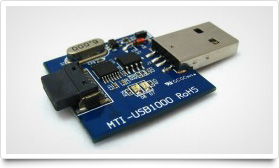
\includegraphics[scale=0.5]{Images/USB1000}
%\end{figure}
%
%\begin{table}[H]
%	\centering
%	\begin{tabularx}{\linewidth}{| l | l | X |}
%	\hline
%	\textbf{Item} & \textbf{Specification} & \textbf{Description} \\
%	\hline
%	\hline
%
%	\multicolumn{3}{|l|}{\textbf{Components}} \\
%	\hline
%	Interface Type & USB type A & USB 1.1 compatible. USB full speed support (12Mbps)\\
%	\hline
%	USB2UART Chip & FTDI\textregistered~ FT232BM & USB2UART converter chip\\
%	\hline
%	1kbit EEPROM & Microchip\textregistered~ 93C46 & Driver ID storage\\
%	\hline
%	Quad Buffer & Texas Instruments\textregistered~ SN74HC126 & USB Rx/Tx Communications buffer\\
%	\hline
%	Octal Switch & Analog Devices\textregistered~ ADG715 & Reset sequence recognition\\
%	\hline
%	Mote Interface & Terminal Block (ERNI\textregistered~ compatible) & Connector to CMXX00 WSN Motes (Vcc, GND, 8 port ADC, 2 port GPIO pins)\\
%	\hline
%
%	\end{tabularx}
%	\caption{Specifications for the USB1000 Interface Board \cite{USB1000}}
%	\label{tab:USB1000-spec}
%\end{table}
%
%\clearpage

\subsection{Sensor Board: CM5000}

\begin{figure}[H]
\centering
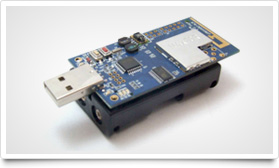
\includegraphics[scale=0.5]{Images/CM5000}
\end{figure}

\begin{table}[H]
	\centering
	\begin{tabularx}{\linewidth}{| l | l | X |}
	\hline
	\textbf{Item} & \textbf{Specification} & \textbf{Description} \\
	\hline
	\hline

	\multicolumn{3}{|l|}{\textbf{Processor}} \\
	\hline
	\multirow{2}{*}{Processor Model} & Texas Instruments\textregistered & Texas Instruments\textregistered\\
	~ & MSP430F1611 & MSP430 family\\
	\hline
	\multirow{3}{*}{Memory} & 48KB & Program Flash \\
	~ & 10KB & Data RAM \\
	~ & 1MB & External Flash (ST\textregistered~ M25P80) \\
	\hline
	ADC & 12bit resolution & 8 channels \\
	\hline
	\multirow{2}{*}{Interfaces} & UART, SPI, I2C & Serial Interfaces \\
	~ & USB & External System Interface (FTI\textregistered~ FT232BM) \\
	\hline
	\hline

	\multicolumn{3}{|l|}{\textbf{Radio}} \\
	\hline
	RF Chip & Texas Instruments\textregistered~ CC2420 & IEEE 802.15.4 2.4GHz Wireless Module\\
	\hline
	Frequency Band & 2.4GHz \mytilde 2.485GHz & IEEE 802.15.4 compliant \\
	\hline
	Sensitivity & -95dBm typ & Receive Sensitivity \\
	\hline
	Transfer Rate & 250Kbps & IEEE 802.15.4 compliant \\
	\hline
	RF Power & -25dBm \mytilde 0dBm & Software Configurable \\
	\hline
	\multirow{2}{*}{Range} & \mytilde120m (outdoor) & \multirow{2}{5cm}{Longer ranges possible with optional SMA antenna attached} \\
	~ & 20~\mytilde30m (indoor) & ~ \\
	\hline
	\multirow{3}{*}{Current Draw} & RX: 18.8mA & \multirow{3}{5.5cm}{Lower RF Power Modes reduce consumption} \\
	~ & TX: 17.4mA & ~ \\
	~ & Sleep mode: 1uA & ~ \\
	\hline
	RF Power Supply & 2.1V \mytilde 3.6V & CC2420 Input Power \\
	\hline
	Antenna & Dipole Antenna / PCB Antenna & Additional SMA connector available for extra antenna \\
	\hline
	\hline

	\multicolumn{3}{|l|}{\textbf{Sensors}} \\
	\hline
	Light 1 & Hamamatsu® S1087 Series & Visible Range (560 nm peak sensitivity wavelength)\\
	\hline
	Light 2 & Hamamatsu® S1087 Series & Visible \& Infrared Range (960 nm peak sensitivity wavelength)\\
	\hline
	\multirow{6}{2.5cm}{Temperature \& Humidity} &  \multirow{6}{*}{Sensirion® SHT11} & Temperature Range: -40 \mytilde 123.8 $^\circ$C  \\
	~ & ~ & Temperature Resolution: $\pm$ 0.01 (typical) \\
	~ & ~ & Temperature Accuracy: $\pm$ 0.4 $^\circ$C (typical) \\
	~ & ~ & Humidity Range: 0 \mytilde 100\% RH \\
	~ & ~ & Humidity Resolution: 0.05 (typical) \\
	~ & ~ & Humidity Accuracy: $\pm$ 3 \%RH (typical) \\
	\hline

	\end{tabularx}
	\caption{Specifications for the CM5000 Wireless Sensor Node \cite{CM5000}}
	\label{tab:CM5000-spec}
\end{table}


\clearpage

\subsection{Network Infrastructure: UD1000}

\begin{figure}[H]
\centering
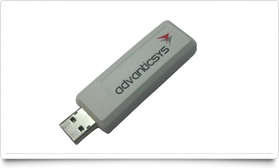
\includegraphics[scale=0.5]{Images/UD1000}
\end{figure}

\begin{table}[H]
	\centering
	\begin{tabularx}{\linewidth}{| l | l | X |}
	\hline
	\textbf{Item} & \textbf{Specification} & \textbf{Description} \\
	\hline
	\hline

	\multicolumn{3}{|l|}{\textbf{Processor}} \\
	\hline
	Processor Model & Texas Instruments\textregistered~ MSP430F1611 & Texas Instruments\textregistered~ MSP430 family\\
	\hline
	\multirow{2}{*}{Memory} & 48KB & Program Flash \\
	~ & 10KB & Data RAM \\
	\hline
	ADC & 12bit resolution & 8 channels \\
	\hline
	\multirow{2}{*}{Interfaces} & UART, SPI, I2C & Serial Interfaces \\
	~ & USB & External System Interface (FTI\textregistered~ FT232BM) \\
	\hline
	\hline

	\multicolumn{3}{|l|}{\textbf{Radio}} \\
	\hline
	RF Chip & Texas Instruments\textregistered~ CC2420 & IEEE 802.15.4 2.4GHz Wireless Module\\
	\hline
	 Frequency Band & 2.4GHz \mytilde 2.485GHz & IEEE 802.15.4 compliant \\
	\hline
	Sensitivity & -95dBm typ & Receive Sensitivity \\
	\hline
	Transfer Rate & 250Kbps & IEEE 802.15.4 compliant \\
	\hline
	RF Power & -25dBm \mytilde 0dBm & Software Configurable \\
	\hline
	Range & \mytilde40m (outdoor), 15\mytilde20m (indoor) & Dongle orientation dependent \\
	\hline
	\multirow{3}{*}{Current Draw} & RX: 18.8mA & \multirow{3}{4.5cm}{Lower RF Power Modes reduce consumption} \\
	~ & TX: 17.4mA & ~ \\
	~ & Sleep mode: 1uA & ~ \\
	\hline
	RF Power Supply & 2.1V \mytilde 3.6V & CC2420 Input Power \\
	\hline
	Antenna & Ceramic antenna & ~ \\
	\hline
	\hline

	\multicolumn{3}{|l|}{\textbf{Electromechanical Characteristics}} \\
	\hline
	Dimensions & 65mm x 22.5mm x 14mm & Including housing\\
	\hline
	Weight & 15g & ~\\
	\hline
	Power & 5V  & DC over USB\\
	\hline
	Current & 90mA  & Max rated current over USB\\
	\hline
	Operating Temperature & -25$^\circ$C \mytilde +60$^\circ$C & ~\\
	\hline
	Storage Temperature & -40$^\circ$C \mytilde +60$^\circ$C & ~\\
	\hline
	Operating Humidity & 5\% \mytilde 95\% & Non condensing\\
	\hline
	Protection type & IP20 & Non condensing\\
	\hline

	\end{tabularx}
	\caption{Specifications for the UD1000 Sensor Network Sink \cite{UD1000}}
	\label{tab:UD1000-spec}
\end{table}


\newpage

\section{References}
\renewcommand{\refname}{\vspace{-1cm}}
\bibliographystyle{myplainnat}
\bibliography{../References/references}

\end{document}
